\documentclass{beamer}
\usepackage{../../../resources/themes/algolymp-light}

\title{Tablouri unidimensionale}
\subtitle{Probleme cu secvențe}
\author{Andrei Mihai Ciobanu}
\institute{Algolymp Summer School}
\date{}
\titlegraphic{
\includegraphics[width=3cm]{../../../resources/algolymp-logo.png}}
\setbeamertemplate{frame footer}{Algolymp Summer School}

% ================================================================
\begin{document}

\begin{frame}
  \titlepage
\end{frame}

\begin{frame}{Cuprins}
  \tableofcontents[hideallsubsections]
\end{frame}

% ================================================================
\section{Introducere}

\begin{frame}[shrink]{Definiție}
  \begin{block}{Definiție}
    Se numește \textbf{secvență} a vectorului $X$ o succesiune de
    \textbf{elemente consecutive} din $X$, în ordinea din $X$. Orice secvență a unui vector este unic determinată de doi indici $l \leq r$, ai primului, respectiv ultimului element din secvență.
  \end{block}
  \begin{block}{Lungimea unei secvențe}
    Secvența $[l, r]$ are lungimea $r - l + 1$.\\
    Exemplu: $[3, 7]$ are lungimea $7 - 3 + 1 = 5$.
  \end{block}
  \begin{block}{Definiție alternativă}
    O secvență continuă se obține eliminând câteva elemente de la \textbf{începutul} șirului
    (posibil niciunul) și câteva de la \textbf{final} (posibil niciunul).
  \end{block}
  \beginnote{Termenii «continuă» și «contiguă» se folosesc interschimbabil în contextul secvențelor.}
\end{frame}

\begin{frame}{Exemple de secvențe continue}
  \begin{center}
  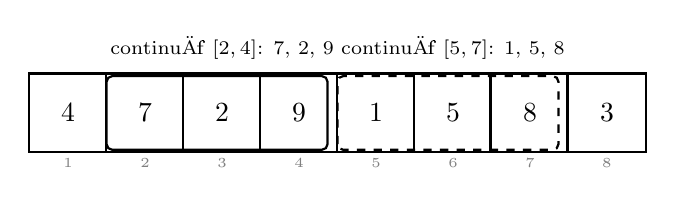
\begin{tikzpicture}[scale=0.85]
    \foreach \i/\v in {1/4, 2/7, 3/2, 4/9, 5/1, 6/5, 7/8, 8/3} {
      \node[draw, thick, minimum width=10mm, minimum height=10mm, fill=white]
        at ({(\i-1)*1.15}, 0) {\v};
      \node[font=\tiny, gray] at ({(\i-1)*1.15}, -0.75) {\i};
    }
    \draw[thick, rounded corners=2pt]
      (0.575, -0.55) rectangle (3.875, 0.55);
    \node[font=\scriptsize, above] at (2.30, 0.65) {continuă $[2,4]$: 7, 2, 9};
    \draw[thick, dashed, rounded corners=2pt]
      (4.025, -0.55) rectangle (7.325, 0.55);
    \node[font=\scriptsize, above] at (5.75, 0.65) {continuă $[5,7]$: 1, 5, 8};
  \end{tikzpicture}
  \end{center}
  \begin{columns}[T]
  \column{0.50\textwidth}
    \begin{block}{Secvențe continue}
      \begin{footnotesize}
      \begin{itemize}\itemsep0pt
        \item $[2,4]$: valorile 7, 2, 9
        \item $[5,7]$: valorile 1, 5, 8
        \item $[4,7]$: valorile 9, 1, 5, 8
        \item $[3,3]$: doar valoarea 2
      \end{itemize}
      \end{footnotesize}
    \end{block}
  \column{0.48\textwidth}
    \begin{alertblock}{Nu sunt continue}
      \begin{footnotesize}
      \begin{itemize}\itemsep0pt
        \item $\{4, 2, 8\}$: poz. 1, 3, 7
        \item $\{7, 9, 5\}$: poz. 2, 4, 6
      \end{itemize}
      \end{footnotesize}
    \end{alertblock}
  \end{columns}
\end{frame}

\begin{frame}{Câte secvențe există într-un șir?}
  \begin{columns}[T]
  \column{0.44\textwidth}
    \begin{center}
    \resizebox{\linewidth}{!}{%
    \begin{tabular}{c p{2.5cm} c}
      \toprule
      Start & Capete posibile \\
      \midrule
      1 & 1, 2, 3, 4, 5 \\
      2 & 2, 3, 4, 5  \\
      3 & 3, 4, 5  \\
      4 & 4, 5  \\
      5 & 5 \\
      \bottomrule
    \end{tabular}}
    \end{center}
  \column{0.54\textwidth}
    \begin{block}{Formula generală}
      \[ 1 + 2 + \cdots + n = \frac{n(n+1)}{2} \]
    \end{block}
    \begin{alertblock}{Problemă}
      La $n = 200{.}000$: circa $2 \times 10^{10}$ secvențe.
      Avem nevoie de metode mai eficiente.
    \end{alertblock}
  \end{columns}
\end{frame}

\begin{frame}[shrink, fragile]{Varianta naivă --- $O(n^3)$}
  \begin{lstlisting}
int n, a[200001]; // ... citire ...
int lmax = 1, rmax = 0;
for (int l = 1; l <= n; l++) {
    for (int r = l; r <= n; r++) {
        bool ok = true;
        for (int k = l; k <= r; k++)
            if (a[k] % 2 == 0) { ok = false; break; }
        if (ok && r - l + 1 > rmax - lmax + 1)
            lmax = l, rmax = r;
    }
}
// lungimea = rmax - lmax + 1
  \end{lstlisting}
  \begin{columns}[T]
  \column{0.48\textwidth}
    \begin{block}{Complexitate: $O(n^3)$}
      Bucla interioară reface verificarea complet.
    \end{block}
  \column{0.50\textwidth}
    \begin{alertblock}{Prea lentă!}
      La $n = 5{.}000$: $\approx 10^{10}$ operații.\\ $\Rightarrow$ Mult prea încet.
    \end{alertblock}
  \end{columns}
\end{frame}

\begin{frame}[fragile]{Varianta de bază --- $O(n^2)$}
  Eliminăm bucla interioară: parcurgem toate perechile $(l, r)$ cu $l \leq r$, extinzând secvența cu câte un element:
  \begin{lstlisting}
int n, a[200001];
// ... citire n si a[1..n] ...

for (int l = 1; l <= n; l++) {
    for (int r = l; r <= n; r++) {
        // prelucreaza secventa a[l..r]
    }
}
  \end{lstlisting}
  \begin{block}{Când este suficientă?}
    Numai când $n \leq 3{.}000$\textendash$5{.}000$.
    Dacă $n = 200{.}000$, avem nevoie de una din metodele din secțiunea următoare.
  \end{block}
\end{frame}

% ================================================================
\section{Diverse abordări}

\subsection{Proprietăți locale}

\begin{frame}[shrink]{O metodă mai bună: proprietăți locale}
  Dacă știu că secvența $[l, r]$ este validă, pot afla rapid dacă $[l, r+1]$ este validă? Dacă \textbf{da}: putem parcurge șirul o singură dată, nefiind nevoie de 2 bucle imbricate.
  \smallskip
  \begin{block}{Exemple în care funcționează}
    \begin{itemize}
      \item Secvențe strict crescătoare: extinderea depinde doar de $a[r]$ și $a[r+1]$; orice subsecvență este de asemenea strict crescătoare
      \item Secvențe de numere prime: depinde doar dacă $a[r+1]$ este prim; orice subsecvență respectă de asemenea această proprietate
    \end{itemize}
  \end{block}
  \begin{alertblock}{Exemplu în care nu funcționează: $\gcd(a[l..r]) > 1$}
    Dacă $\gcd(a[l..r{+}1]) = 1$ (invalid), poate exista $l' > l$ cu $\gcd(a[l'..r{+}1]) > 1$.
    Nu știm unde să resetăm \texttt{len} \textemdash{} nu putem folosi simplu \texttt{len = 1}.
  \end{alertblock}
\end{frame}

\begin{frame}[fragile, shrink]{Secvența strict crescătoare --- $O(n)$}
  Ținem variabila \texttt{len} = lungimea secvenței strict crescătoare care se termină \textbf{acum}.
  La fiecare pas: dacă $a[i-1] < a[i]$, secvența continuă; altfel, reluăm de la 0.
  \begin{lstlisting}
int n, a[200001];
// ... citire ...

int len = 1, best = 1;
for (int i = 2; i <= n; i++) {
    if (a[i-1] < a[i]) {
        len++;           // secventa continua
    } else {
        len = 1;         // secventa s-a rupt, reluam de la i
    }
    if (len > best) {
        best = len;
    }
}
cout << best << "\n";
  \end{lstlisting}
\end{frame}

\begin{frame}{Exemplu --- șirul 1, 3, 5, 2, 3, 6, 7, 8, 4, 9}
  \begin{center}
  \footnotesize
  \begin{tabular}{r|cccccccccc}
    \toprule
    $i$           & 1 & 2 & 3 & 4          & 5 & 6 & 7 & 8          & 9          & 10 \\
    $a[i]$        & 1 & 3 & 5 & 2          & 3 & 6 & 7 & 8          & 4          & 9  \\
    \texttt{len}  & 1 & 2 & 3 & \textbf{1} & 2 & 3 & 4 & 5          & \textbf{1} & 2  \\
    \texttt{best} & 1 & 2 & 3 & 3          & 3 & 3 & 4 & \textbf{5} & 5          & 5  \\
    \bottomrule
  \end{tabular}
  \end{center}
  \begin{block}{Concluzii}
    Pozițiile $4$\textendash$8$: valorile $2, 3, 6, 7, 8$ formează cel mai lung segment. \textbf{Răspuns: 5}.
  \end{block}
  \begin{block}{Problemă: \href{https://code.algolymp.com/problems/4204}{Longest Increasing Contiguous Segment}}
    Determină lungimea maximă a secvenței strict crescătoare continue. $1 \leq n \leq 200{.}000$.
  \end{block}
\end{frame}

\begin{frame}[fragile, shrink]{Numărarea segmentelor cu o proprietate}
  \begin{block}{Observație}
    Dacă secvența cu proprietatea $P$ curentă are lungimea \texttt{len},
    atunci exact \texttt{len} astfel de secvențe se termină la $i$.
  \end{block}
  \begin{block}{Exemplu: șirul 2 4 7, proprietatea ``strict crescător''}
    Secvențele strict crescătoare ce se termină la 7:
    $[7]$, $[4,7]$, $[2,4,7]$ \textemdash{} total 3 = \texttt{len}.
  \end{block}
  \begin{lstlisting}
long long answer = 0;
int len = 1;
for (int i = 1; i <= n; i++) {
    if (i > 1 && a[i-1] < a[i]) {
        len++;
    }
    else {
        len = 1;
    }
    answer += len;
}
cout << answer << "\n";
  \end{lstlisting}
  \beginnote{Numărul de secvențe poate fi circa $n^2/2$; folosește \texttt{long long} pentru \texttt{answer}}
\end{frame}

% ================================================================
\subsection{Secvența de sumă maximă}

\begin{frame}{Secvența de sumă maximă}
  \begin{block}{Problemă}
    Găsește secvența cu suma maximă (elementele pot fi negative).
  \end{block}
  \begin{block}{Algoritmul lui Kadane}
    Fie \texttt{current} = suma maximă a secvenței care se termină la poziția $i$.\\[3pt]
    \textbf{Dacă \texttt{current} $< 0$}: orice prelungire a prefixului curent e mai slabă
    decât una care începe proaspăt. Resetăm \texttt{current = 0}.\\[3pt]
    \textbf{Altfel}: extindem cu $a[i]$.
  \end{block}
  \begin{block}{Complexitate: $O(n)$, memorie $O(1)$}
    O singură parcurgere; variabilele \texttt{current} și \texttt{best}.
  \end{block}
\end{frame}

\begin{frame}[fragile]{Secvența de sumă maximă --- implementare}
  \begin{lstlisting}
int n, a[200001];
// ... citire ...
int best = a[1], current = a[1];
for (int i = 2; i <= n; i++) {
    if (current < 0) {
      current = 0;
    }
    current += a[i];
    if (current > best) {
        best = current;
    }
}
cout << best << "\n";
  \end{lstlisting}
  Inițializarea \texttt{best = a[1]} (nu $0$) tratează corect cazul
  în care toate elementele sunt negative.
\end{frame}

% ================================================================
\subsection{Sliding Window}

\begin{frame}[fragile, shrink]{Sliding Window}
  \begin{block}{Problemă}
    Calculează suma fiecărei secvențe de lungime exact $k$.
    Variantă directă: $O(n \cdot k)$. Putem face $O(n)$.
  \end{block}
  Când fereastra se mută cu un pas la dreapta, iese $a[\text{left}-1]$
  și intră $a[\text{left}+k-1]$:
  \begin{lstlisting}
long long sum = 0;
for (int i = 1; i <= k; i++) sum += a[i]; // prima fereastra [1,k]
// prelucreaza fereastra [1, k]

for (int left = 2; left + k - 1 <= n; left++) {
    sum -= a[left - 1];      // iese din stanga
    sum += a[left + k - 1];  // intra din dreapta
    // prelucreaza fereastra [left, left+k-1]
}
  \end{lstlisting}
  \begin{block}{Complexitate: $O(n)$}
  \end{block}
\end{frame}

% ================================================================
\subsection{Sume parțiale}

\begin{frame}[fragile]{Sume parțiale: câte secvențe de lungime $K$ au suma $\leq X$?}
  \begin{block}{Idee}
    Suma secvenței $[l, l{+}K{-}1]$ = $\texttt{pref}[l+K-1] - \texttt{pref}[l-1]$.
    Iterăm $l$ de la $1$ la $n{-}K{+}1$ și numărăm câte satisfac condiția.
  \end{block}
  \medskip
  \begin{lstlisting}
// pref[0] = 0, pref[i] = pref[i - 1] + a[i]
int answer = 0;
for (int l = 1; l + k - 1 <= n; l++) {
    if (pref[l + k - 1] - pref[l - 1] <= x) {
        answer++;
    }
}
cout << answer << "\n";
  \end{lstlisting}
  \textbf{Complexitate:} $O(n)$ (precalculare + numărare)
\end{frame}

% ================================================================
\subsection{Căutare binară}

\begin{frame}{Căutare binară pe sume parțiale}
  \begin{block}{1. Împărțire în 2 secvențe de sume egale --- $O(n)$}
    Fie $S = \texttt{pref}[n]$. Tăietura la $i$ este validă dacă $\texttt{pref}[i] = S/2$.
    Iterăm $i \in [1, n{-}1]$ și numărăm.
  \end{block}
  \begin{block}{2. Împărțire în 3 secvențe de sume egale --- $O(n \log n)$}
    Fixăm prima tăietură la $i$: $\texttt{pref}[i] = S/3$.
    Căutăm binar a doua tăietură $j \in [i{+}1, n{-}1]$ cu $\texttt{pref}[j] = 2S/3$.\\
    \textit{(Necesită $a[i] \geq 0$, altfel sumele parțiale nu sunt crescătoare.)}
  \end{block}
  \begin{alertblock}{3. Împărțire în 4 secvențe}
    Hint: cum putem adapta ideea de la problema 2?
  \end{alertblock}
\end{frame}

\begin{frame}[shrink, fragile]{Împărțire în 3 secvențe de sume egale --- implementare}
  \begin{lstlisting}
// S = pref[n], necesita S % 3 == 0 si a[i] >= 0
int answer = 0;
for (int i = 1; i <= n - 2; i++) {
    if (3 * pref[i] != S) {
        continue;
    }
    // ... cautam binar j ...
    if (pref[j] == 2 * S / 3) {
        answer++;
    }
}
cout << answer << "\n";
  \end{lstlisting}
  \textbf{Complexitate:} $O(n \log n)$; atenție cand valorile pot fi nule $\Rightarrow$ $j$ poate avea mai multe valori valide

    Generalizare: $K$ secvențe $\Rightarrow$ $K{-}1$ tăieturi, căutăm binar fiecare $\Rightarrow O(K \log n)$ (doar pentru valori pozitive).
\end{frame}

% ================================================================
\subsection{Pattern matching}

\begin{frame}[shrink, fragile]{Pattern matching}
  \begin{block}{Problemă: \href{https://code.algolymp.com/problems/4205}{Pattern Inside a Sequence}}
    Se dau șirul $a$ (lungime $n$) și șablonul $b$ (lungime $m$).
    Numără câte poziții de start $i$ au proprietatea că $a[i..i{+}m{-}1] = b[1..m]$.\\
    \textbf{Restricții:} $1 \leq m \leq n \leq 3{.}000$.
    \textbf{Exemplu:} $a{=}[1,2,1,2,1]$, $b{=}[1,2,1]$ $\Rightarrow$ răspuns 2.
  \end{block}
  \begin{lstlisting}
int n, m, a[3001], b[3001], answer = 0;
for (int start = 1; start + m - 1 <= n; start++) {
    bool ok = true;
    for (int j = 1; j <= m; j++) {
        if (a[start + j - 1] != b[j]) {
            ok = false;
            break;
        }
    }
    if (ok) {
        answer++;
    }
}
cout << answer << "\n";
  \end{lstlisting}
  Complexitate: $O(n \cdot m)$, acceptabilă pentru $n, m \leq 3{.}000$.
\end{frame}

% ================================================================
\subsection{Two Pointers}

\begin{frame}{Two Pointers --- tema lecției următoare}
  \begin{block}{Când Sliding Window nu este suficient}
    Sliding Window funcționează pentru lungime \textbf{fixă} $k$.
    Two Pointers = fereastră cu lungime variabilă.
  \end{block}
  \begin{block}{Problemă: secvența de lungime maximă cu suma $\leq K$}
    Ținem doi indici $l \leq r$. Extindem $r$ la dreapta; dacă suma depășește $K$,
    avansăm $l$. Fiecare index se mișcă cel mult $n$ pași: $O(n)$ total.
  \end{block}
  \begin{block}{Condiție de aplicabilitate}
    Proprietatea trebuie să fie \textbf{monotonă}: dacă $[l,r]$ e validă, atunci
    $[l, r{-}1]$ e de asemenea validă.
  \end{block}
\end{frame}

% ================================================================
\section{Recapitulare}

\begin{frame}{Probleme de antrenament}
  \begin{enumerate}
    \item \href{https://code.algolymp.com/problems/4204}{\textbf{Longest Increasing Contiguous Segment}}
    \item \href{https://code.algolymp.com/problems/4205}{\textbf{Pattern Inside a Sequence}}
    \item \href{https://code.algolymp.com/problems/1929}{\textbf{seism}} (OJI 2021 VI)
    \item \href{https://code.algolymp.com/problems/3572}{\textbf{mandatar}} (OJI 2025 VI)
    \item \href{https://code.algolymp.com/problems/2996}{\textbf{Avid}} (OJI 2024 VI)
    \item \href{https://code.algolymp.com/problems/3853}{\textbf{zudt}} (OJI 2026 VI)
  \end{enumerate}
\end{frame}

\begin{frame}{Resurse}
  \begin{enumerate}
      \item \href{https://www.pbinfo.ro/articole/5613/secvente-in-vectori}{\textbf{pbinfo} --- Secvențe în vectori}
          \textemdash{} definiție, complexități O($n^3$)/O($n^2$)/O($n$), exemple C++
    \smallskip
    \item \href{https://www.pbinfo.ro/articole/20499/secventa-de-suma-maxima}{\textbf{pbinfo} --- Secvența de sumă maximă}
          \textemdash{} algoritmul lui Kadane explicat pas cu pas
  \end{enumerate}
\end{frame}

\end{document}
